
\begin{figure*}[ht!]
\centering
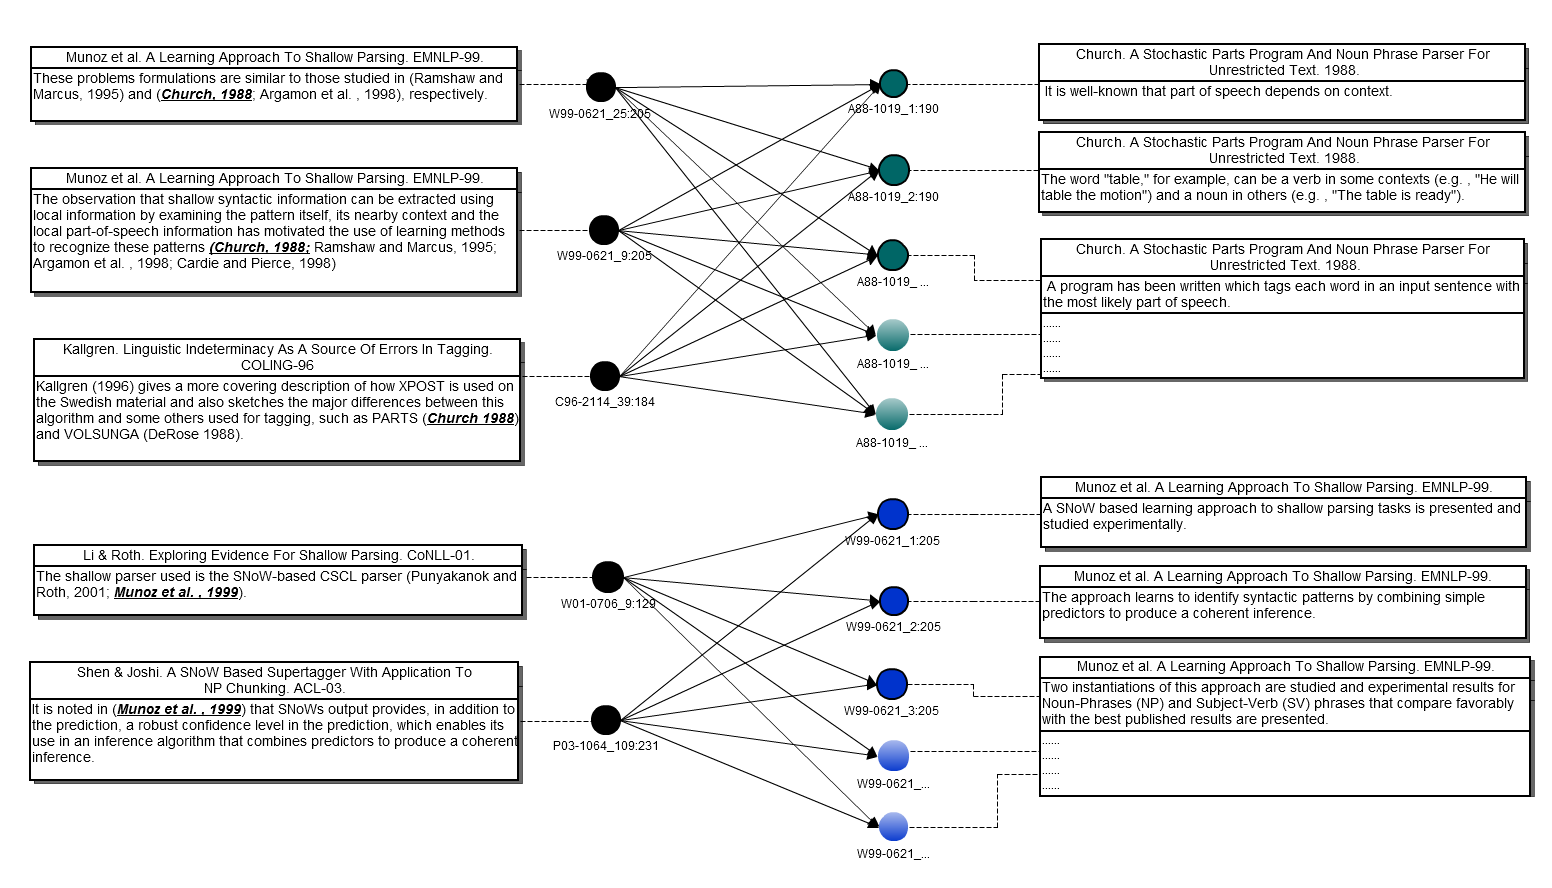
\includegraphics[width=\textwidth]{graph/bipartite_graph.png}
\caption{A mini-model of the bi-partite graph for Chapter 5 (Part-of-Speech Tagging)}\label{fig:bi}
\end{figure*}

\begin{table*}
\centering
{\scriptsize
\begin{tabular}{|l|cc|rrr|}
  \hline
 Chapter & src & cit & $|\B_L|$ & $|\B_R|$ & $E_\B$ \\
  \hline \hline
 Words and Transducers & 14&     255&    489&    $3,484$ &   $202,940$ \\
 N-grams & 5&      73&     97&     $2,083$ &   $32,690$ \\
 Part-of-Speech Tagging & 16&     657&    $1,261$ &   $3,385$ &   $344,886$\\
 Hidden Markov and Maximum Entropy Models & 2&      432&    659&    525&    $187,905$\\
 Phonetics & 1&      12&     81&     216&    $17,496$\\
 Speech Synthesis & 4&      54&     126&    920&    $29,357$\\
 Automatic Speech Recognition & 2&      27&     103&    401&    $21,566$\\
 Speech Recognition: Advanced Topics & 7&      189&    445&    $2,007$&   $96,467$\\
 Syntactic Parsing & 4&      131&    246&    763&    $63,673$\\
 Dialog and Conversational Agents & 11&     170&    368&    $3,745$ &   $114,281$\\
  \hline
\end{tabular}}
\caption{List of chapter historical notes used in our experiments together with the number of source papers extracted from historical notes (src), the number of citing papers extracted from AAN (cit), size of the left ($\B_L$) and right ($\B_R$) components in the bi-partite graph, and number of edges in the graph ($E_\B$).}\label{tbl:chapters}
\end{table*}

\section{Approach}
\label{sec:approach}

Previous work on scientific survey generation have compared surveys that are generated from different sources such as citations and source paper texts~\cite{Qazvinian&Radev08a,mei&zhai08,mohammad-EtAl:2009:NAACLHLT09}. However, none of these approaches combine these heterogeneous information sources to produce automatic surveys. 

In our approach, we investigate the usefulness of combining different information sources and producing summaries that are both affected by source paper text and citation information. For a set of papers in the same scientific topic, we extract survey worthy sentences from the source texts that cover contributions recognized by other scholars in citations, and extract citations that cover contributions that are recognized by the authors in the source text.

In our algorithm, we model the set of papers in a scientific topic $t$ as a bi-partite graph, $\B$ with a left and a right component ($\B_L$, $\B_R$). Each node in $\B_L$ is a citation sentence to one or more papers in $t$ extracted from AAN, and each node in $\B_R$, represents a sentence extracted from the source text of a paper in $t$. We construct the edges in $\B$ by connecting each citing sentence to all the source sentences in the papers it cites. Each edge in $\B$ is assigned a weight equal to the cosine similarity of the TF-IDF term vectors of the two sentences it connects. 
Figure~\ref{fig:bi} illustrates part of the bi-partite graph for built for the ``Part-of-Speech Tagging'' chapter in the JM book.

To build the summaries we are interested in citations and source sentences that cover important contributions in the given scientific topics. Intuitively, contributions that both the paper authors and other scholars recognize as significant are important and should be extracted. Surveyor extracts citations that cover important contributions mentioned in the source papers as well as source sentences that discuss important factoids recognized by others in citations.


\subsection{Ranking}
The inherent duality in the source papers and citations suggests that the problem could be addressed by applying the HITS algorithm~\cite{Kleinberg:1999} to iteratively assign hub and authority scores to citations and source sentences respectively. The induction process is as follows. Each citation sentence $c\in \B_L$ is associated with a hub score $h_c$, and each source sentence $s\in \B_R$ is associated with an authority score $a_s$. These scores are initialized with a value of $1.0$.  Hub and authority scores are iteratively updated using the following equations.

{\small
\begin{eqnarray}
\label{hits1} a^{(i+1)}_s = \sum_{c\in nei(s)} \frac{h^{(i)}_c}{H^{(i)}}
\end{eqnarray}
}
{\small
\begin{eqnarray}
\label{hits2} h^{(i+1)}_c = \sum_{s\in nei(c)} \frac{a^{(i)}_s}{A^{(i)}}
\end{eqnarray}
}

where a source sentence $s$ is in a citation sentence, $c$'s neighborhood ($s\in nei(c)$) if there is an edge between $s$ and $c$ in $\B$ ($c$ cites the paper that contains $s$), and their cosine similarity is greater than a threshold (i.e., $cos(s,c) > \theta$). Here, $H^{(i)}$ and $A^{(i)}$ are normalization factors:

{\small
\begin{eqnarray}
H^{(i)} = (\sum_{c\in \B_L} {h^{(i)}_c}^2)^{1/2}\\
A^{(i)} = (\sum_{s\in \B_R} {a^{(i)}_s}^2)^{1/2}
\end{eqnarray}}

In our experiments, we set $\theta = 0.1$. This ranking gives us top authorities (source sentences) and top hubs (citations) with which we build two different summaries: {\bf $\textrm{HITS}_\textrm{src}$} and {\bf $\textrm{HITS}_\textrm{cit}$}. Although these summaries are built from different sources (i.e., source papers and citations) they are affected by each other. In other words, the scores and thus extraction of top citations affects the extraction of top source sentences and vice versa. 


\subsection{Adding Weights}
In previous section, we described the basic version of our system in which the edges are considered as binary connections (if the cosine similarity is above a threshold). We would like to investigate the effect of similarity on sentence extraction. In other words, instead of applying a threshold we use the actual edge weights and modify Equations \ref{hits1}, \ref{hits2} as follows.

{\small
\begin{eqnarray}
\label{whits1} a^{(i+1)}_s = \sum_{c\in nei(s)} \frac{w_{cs} \cdot  h^{(i)}_c}{H^{(i)}}\\
\label{whits2} h^{(i+1)}_c = \sum_{s\in nei(c)} \frac{w_{sc} \cdot a^{(i)}_s}{A^{(i)}}
\end{eqnarray}}

where $w_{sc}$ is the is the edge weight between vertices $s$ and $c$, calculated as the TF-IDF based cosine similarity between their corresponding sentences.

Intuitively, this modification will take into account the similarity of sentence with its neighbors rather than the number of connections, and would result in summaries that contain more \emph{lexically} salient sentences. 
The weighted ranking gives us top authorities (source sentences) and top hubs (citations) with which we build two different summaries: {\bf $\textrm{HITS}_\textrm{src} \textrm{ with weights}$} and {\bf $\textrm{HITS}_\textrm{cit} \textrm{with weights}$}.

\subsection{Citation Bias}
The downside of the current HITS-based sentence extraction is that it assumes equal importance for the papers in a given topic. However, contributions from highly cited papers are intuitively more important. To address this issue, we propose an improvement inspired by~\cite{Mei&al2010} and modify equations \ref{hits1}, \ref{hits2} to include a prior distribution of prestige.

{\small
\begin{eqnarray}
\label{phits1} a^{(i+1)}_s = (1- \lambda) \cdot p^\ast(s) + \lambda \cdot \sum_{c\in nei(s)} \frac{w_{cs}\cdot h^{(i)}_c}{H^{(i)}}\\
\label{phits2} h^{(i+1)}_c = (1- \lambda) \cdot p^\ast(c) + \lambda \cdot \sum_{s\in nei(c)} \frac{w_{sc}\cdot a^{(i)}_s}{A^{(i)}}
\end{eqnarray}}

Here, $p^\ast(v)$ is a distribution which represents the prior preference of vertex $v$. When $p^\ast(v)$ is uniform, the left component is similar to the random jumping probabilities in PageRank. Other possible choices for $p^\ast(v)$ include a topic sensitive distribution, inspired by personalized jumping in personalized PageRank~\cite{Haveliwala2002,haveliwala2003topic}. 
In Equations~\ref{phits1},~\ref{phits2} $\lambda$ obtains a value between $0$ and $1$. When $\lambda = 1$, Equations~\ref{phits1},~\ref{phits2} lead to the standard HITS algorithm. In our experiments, we set $\lambda = 0.75$. 

The prior distribution allows us to favor citation sentences that are from more impactful papers. Therefore we define the prior distributions as the normalized citation frequency of the paper 

{\small
\begin{eqnarray}
p^\ast (v) = \frac{C_v + 1}{\sum_{v\in \B} C_v + |\B|} 
\end{eqnarray}}

where $C_v$ is the number of citations to the paper that contains sentence $v$.  
Equations~\ref{phits1},~\ref{phits2} give us top authorities (source sentences) and top hubs (citations) with which we build two different summaries:  {\bf $\textrm{HITS}_\textrm{src} \textrm{ with weights/priors}$} and {\bf $\textrm{HITS}_\textrm{cit} \textrm{with weights/priors}$}. 

